% 来源：OEBPS/Text/Section0001_split_007.xhtml#sigil_toc_id_49

\BookChapter{36}
\section[第36章\q 保罗·都铎·琼斯：当代罗宾汉]{第36章\\ 保罗·都铎·琼斯：当代罗宾汉}

\begin{figure}[htbp]
\centering
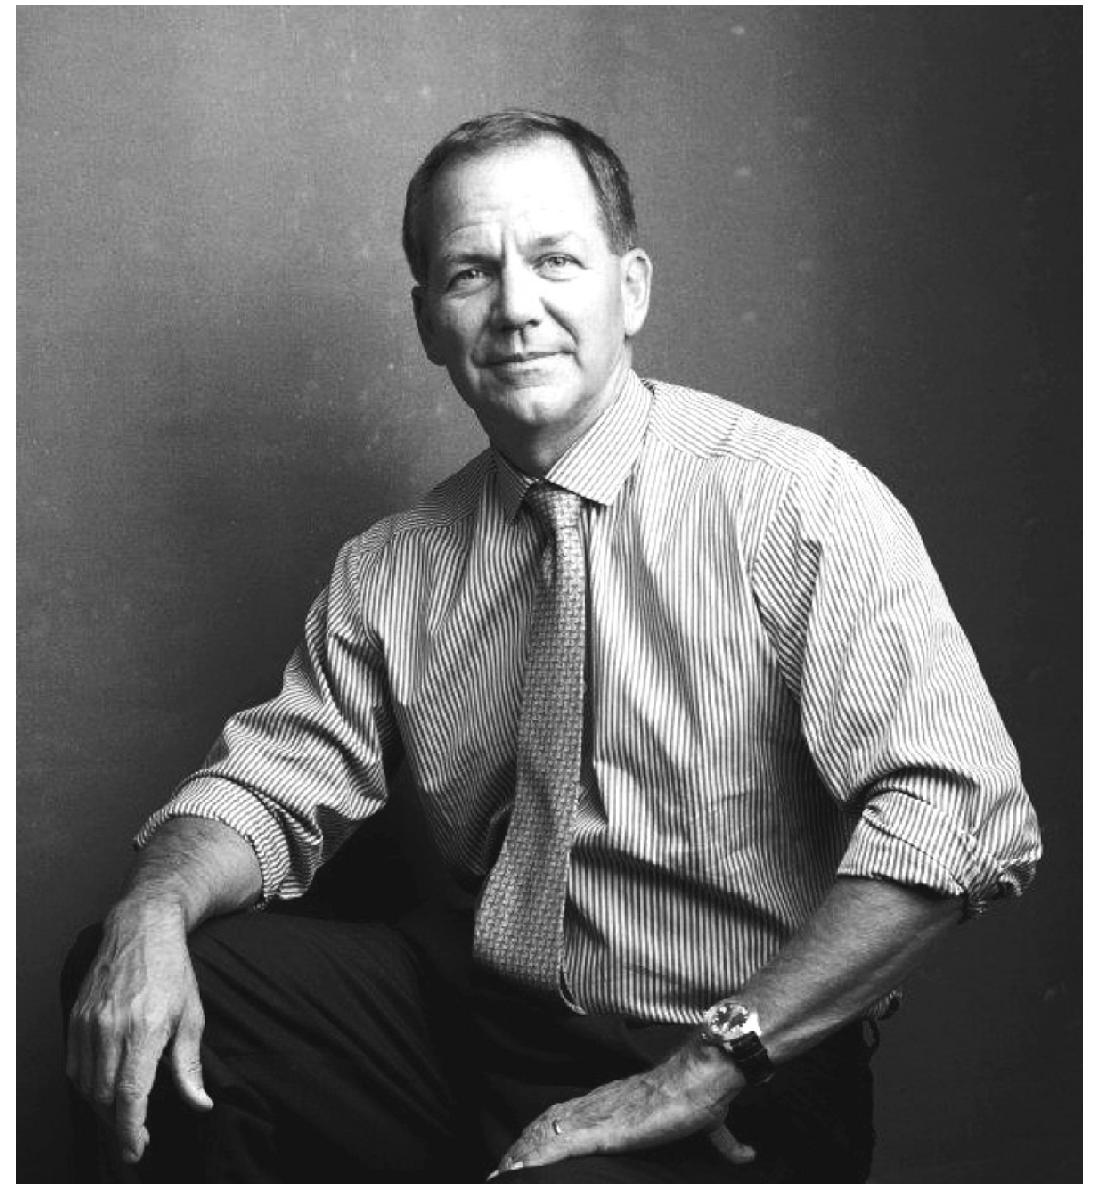
\includegraphics[width=0.43\linewidth,keepaspectratio]{image/保罗·都铎·琼斯肖像.jpg}
\caption*{保罗·都铎·琼斯}
\end{figure}

都铎投资公司创始人，罗宾汉基金会创始人

保罗·都铎·琼斯是有史以来最成功的交易员之一，26岁创办自己的企业，在此之前他在大宗商品期货市场做棉花交易，白手起家。

保罗·都铎·琼斯好像完全违反了重力法则，连续28年，年年盈利。这个人还是个成功预测到“黑色星期一”的传奇人物。1987年股市大崩盘，一天暴跌22\%，创下有史以来最大单日跌幅。2008年，当全世界都深陷在股市大崩盘的痛苦之中时，保罗·都铎·琼斯的对冲基金却获得了60\%的单月收益率，这一年的收益率接近200\%。

保罗·都铎·琼斯是我的密友，也是我的个人英雄偶像，我非常荣幸，从1993年起一直担任他的巅峰表现教练，在他创下连续28个年度赚钱的传奇过程中，其中21年我都陪伴左右，和他共度大半个交易生涯。比起保罗·都铎·琼斯令人震惊的投资成功，我印象更深刻的是，他发自内心地痴迷于不断寻找合适的方式回馈社会，为推动社会发展进步而努力。保罗·都铎·琼斯创办了著名的罗宾汉基金会，激发和组合一些全世界最聪明和最富有的投资者互相合作，与纽约市的贫穷问题开战。保罗·都铎·琼斯和他的罗宾汉团队做这份慈善工作，也是尽力做出非常严谨的分析——那些对冲基金的亿万富翁本来只在投资上才肯下这么大的功夫。从1988年起，罗宾汉基金会已经投资了14.5亿美元用于解决纽约市贫穷问题的项目，就像在投资上无情地追求风险—收益不对称一样（下文将分享他的1∶5风险—收益不对称投资原则），保罗·都铎·琼斯的基金会做慈善工作也没有什么不同。罗宾汉基金会的运作和管理成本百分之百地由董事会委员自掏腰包，所以，捐赠者投资于自己所在社区的慈善项目能得到15∶1的收益率！正如谷歌公司的执行董事长埃里克·施密特所说的：“简直就像没有基金会，没有搞活动，却更有效果。”

保罗·都铎·琼斯会告诉你，他是一个交易员，不是传统的投资者，但是就像他的前任老板E. F. 赫顿一样，保罗·都铎·琼斯一说话，人人就会侧耳恭听。作为一个宏观交易者，他研究了很多影响因素：基本面、心理、技术分析、资金流动、世界性的大事件，以及它们对资产价格的影响。保罗·都铎·琼斯不关注个股，他赌的是影响整个世界格局的大趋势，比如，从美国到中国、从货币到大宗商品再到利率。很多全世界最有影响力的领导人都向他寻求指导和帮助，其中包括财政部部长、央行官员、全世界各国政府的智囊团。

我和保罗·都铎·琼斯这次会谈的地点在他的公司办公园区里，那里面积很大，坐落在康涅狄格州格林尼治市，都铎投资舰队都在这里办公。会谈期间，我们深度探讨了最有价值的投资原则，他要分享给大家，让你我这样的个人投资者能够从中受益。结果一番长谈之后，保罗·都铎·琼斯要送给我们的是他的“价值10万美元的商业投资课程”，原来每年能够听到他这个课程的只有他们公司的交易员，以及极少数非常幸运的大学生。保罗·都铎·琼斯的所有投资智慧都浓缩在下面短短几页的文字里。

\begin{BookQuote}
\textbf{罗宾斯：}保罗，你在投资上，在交易上，都可以说是连续28年盈利，没有一年亏钱，这简直难以置信，你是怎么做到的？
\end{BookQuote}

\begin{BookQuote}
\textbf{保罗·都铎·琼斯：}我们都是环境的产物，环境造就人。我是1976年进入金融行业的，一开始做大宗商品交易员，交易棉花、大豆、橙汁等，最重要的事情是，这些市场很大程度上会受到大气候的影响。只需三四年的时间，你就会经历巨大的牛市和巨大的熊市。我很快搞懂了牛市和熊市的心理，它们的转变能有多快？当市场跌到谷底的时候，市场的情绪是什么样的？我看到有人先赚到巨大的财富又全部亏掉。我就坐在那里，亲眼看着邦克·亨特大买白银4亿美元，到1980年涨到100亿美元，这让他一下子成了世界首富，后来只过了5个星期，他就从100亿美元又跌回到了4亿美元。
\end{BookQuote}

\begin{BookQuote}
\textbf{罗宾斯：}啊！
\end{BookQuote}

\begin{BookQuote}
\textbf{保罗·都铎·琼斯：}这样我就一下子知道了，钱去得有多快。你能拥有财富的时候，一定要知道这是多么宝贵。从那件事上我学到的最重要东西是，防守比进攻重要10倍。你拥有的财富，很容易像刮大风一样一下子就没了，你必须非常小心下行风险，任何时候都要小心。
\end{BookQuote}

\begin{BookQuote}
\textbf{罗宾斯：}必须。
\end{BookQuote}

\begin{BookQuote}
\textbf{保罗·都铎·琼斯：}如果你有一笔投资涨得很好，那你根本不用管它，它会自己照顾好自己的。你需要非常关注的是正在亏钱的投资，可是事实上大家往往看都不愿意看正在亏钱的投资：“我的账户正在下跌，我甚至都不愿意打开它。”所以长期下来，我创造出一个流程，让我关注的最重要的单一因素就是风险控制，每天都是这样。我想知道如何不亏损。
\end{BookQuote}

\begin{BookQuote}
\textbf{罗宾斯：}你认为普通投资大众关于投资最大的误区是什么？什么样的投资误区损害了他们？
\end{BookQuote}

\begin{BookQuote}
\textbf{保罗·都铎·琼斯：}你能投资很长时间，但你要变得富有并不是非得用很长时间。因为市场上每样东西都有价格，长期来看也有一个中心价值，找到那些价格过分低于中心价值的品种，你就能赚到大钱，这不一定需要很长时间。但是我认为，这要求普通投资者明白那些一直适用的估值指标，你一定要防备好估值出错，因为事实上你并不是对每一种资产类型都了解，预防出错的办法就是建立一个非常分散的投资组合。
\end{BookQuote}

\begin{BookQuote}
\textbf{罗宾斯：}你说得很对。
\end{BookQuote}

\begin{BookQuote}
\textbf{保罗·都铎·琼斯：}有个故事，我永远不会忘记，那是1976年，我才工作了6个月，我去见我的老板伊莱·塔利斯，他是一个棉花期货交易员。我说：“我要做交易，我要做交易。”他说：“孩子，现在，你还不能做交易，也许再过6个月，我会让你做交易。”我说：“不，不，不！我现在就要做交易。”他说：“现在你给我听着，再过30年，市场肯定还在，问题是你还在不在！”
\end{BookQuote}

\begin{BookQuote}
\textbf{罗宾斯：}这个问题问得太好了。
\end{BookQuote}

\begin{BookQuote}
\textbf{保罗·都铎·琼斯：}所以龟兔赛跑最后是乌龟赢了，对不对？我想，你能做的最重要的一件事就是把你的投资组合分散投资。分散是关键，搞好防守是关键，那我要再说一次，还有，一直留在比赛里，能待多久就待多久，剩者为王。
\end{BookQuote}

\begin{BookQuote}
\textbf{罗宾斯：}按照分散投资的原则，那么你看，要做好防守，应该怎么做资产配置才行？
\end{BookQuote}

\begin{BookQuote}
\textbf{保罗·都铎·琼斯：}从来不会有这样的时候，你可以绝对肯定地说，这样配置的投资组合我能一直持有5\textasciitilde{}10年。这是不可能的。现在这个世界发展变化得太快了。你现在看一看，美国的股票和债券都被高估得简直荒谬可笑。现金一文不值，活期存款利率相当于零，你手里的钱该用来做什么？有的时候应该拿着现金，有的时候应该做投资。你并不需要总是能有机会赚大钱，耐心等待，赚大钱的机会并不是想有就有的，也并不是经常有的。
\end{BookQuote}

\begin{BookQuote}
\textbf{罗宾斯：}那么你是怎么做的？
\end{BookQuote}

\begin{BookQuote}
\textbf{保罗·都铎·琼斯：}有的时候，你只能说：“哎呀，这里根本没有价值，那里一点儿都没有吸引力。我要做好防守，配置一个投资组合，没有很大的盈利预期，但关键是不要亏损。我会做一些投资，肯定不会让自己受到损失的投资，将来如果市场的投资价值增长了，我还有资本抓住一些机会。”
\end{BookQuote}

\begin{BookQuote}
\textbf{罗宾斯：}那么你用什么具体的策略来保护你的投资组合？
\end{BookQuote}

\begin{BookQuote}
\textbf{保罗·都铎·琼斯：}我在弗吉尼亚大学给本科生上课，我告诉那些来听课的学生：“你不用去商学院读工商管理硕士了，我能给你省一大笔学费。现在你就能得到价值10万美元的一堂课，只需要记住我说的两点就够了：你一定要跟上最重要的大趋势；做逆向投资者，你想都不要想。美国两个最有钱的人——巴菲特和比尔·盖茨，他们是怎么赚到那么多钱的？比尔·盖茨能赚到那么多钱，是因为他一直拥有一只股票，就是他创立的微软，这只股票涨了800倍，他一直跟着大趋势走。巴菲特呢，他说“我要买伟大的公司，我会一直持有这些公司的股票，我不会卖，因为这才是既正确又精明的做法，只要我不卖，一直拿住，复利法则就会为我工作，给我创造巨大的复利增长。
\end{BookQuote}

\begin{BookQuote}
\textbf{罗宾斯：}还有巴菲特控股的保险公司有巨大的现金流，能给他提供投资所需要的巨额资金。
\end{BookQuote}

\begin{BookQuote}
\textbf{保罗·都铎·琼斯：}巴菲特就这样一直握着那些大公司的股票，坐在那里一动不动，经历了人类文明史上最大的牛市。巴菲特抵抗住了忍不住想要兑现盈利的痛苦。
\end{BookQuote}

\begin{BookQuote}
\textbf{罗宾斯：}巴菲特太了不起了。所以，我的下一个问题是，你怎么判定未来的大趋势？
\end{BookQuote}

\begin{BookQuote}
\textbf{保罗·都铎·琼斯：}我对任何投资的衡量标准都是看200日收盘价格移动平均线。我看到过很多东西最终价格都归于零，股票是这样的，大宗商品也是这样的。投资的全部技巧都在这一点上：“我怎么避免亏个精光？”如果你用200日移动平均线，你就能避免亏个精光了。做好防守，你就能避免亏个精光。我在大学里给学生上技术分析课程的时候，我会让学生做这种练习。我会画一个假设的走势图，像下边这个图一样，在白板上贴一张白纸，画上一根走势线，一直上涨，涨到最高的地方，纸上都画不下了。
\end{BookQuote}

\begin{figure}[htbp]
\centering
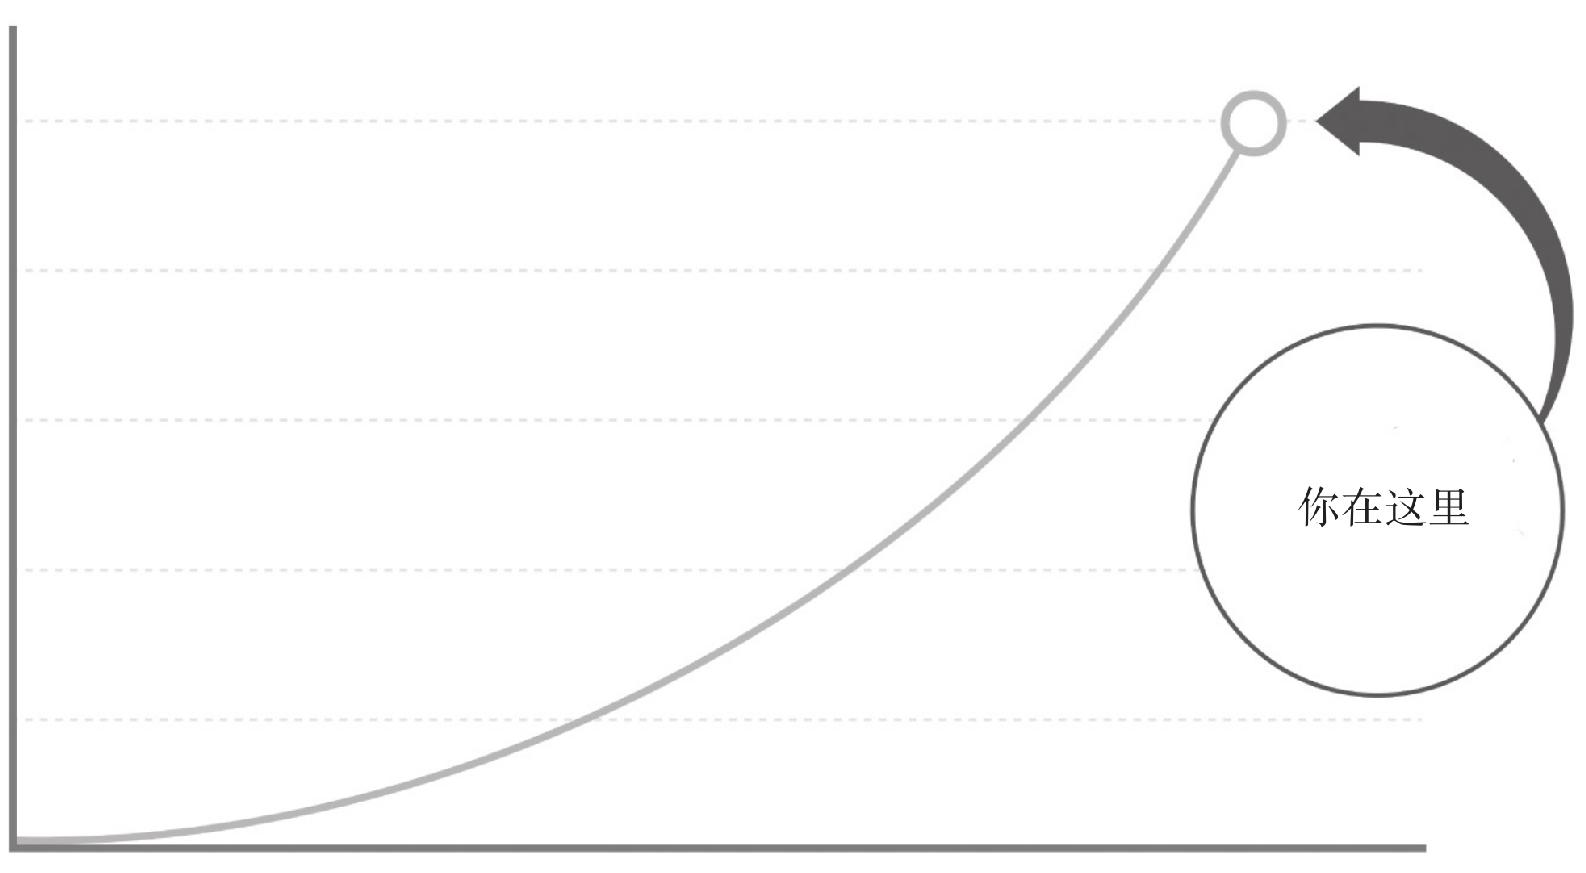
\includegraphics[width=0.76\linewidth,keepaspectratio]{image/36-1.jpg}
\caption{}\label{fig:36-1}
\end{figure}

画好之后，我会问学生：“好啦，你知道的就是现在你看到的。有多少人会看涨，而且继续看涨呢？请举手。”一般会有60\%的人举手。我再问：有多少人会看跌，会卖出这些投资呢？一般会有40\%左右的人举手表示愿意卖出。然后我说：“你们这40\%想要卖出的人这辈子永远不要用你自己的钱做投资，因为你的脑子里有逆向投资的漏洞。本来有可能赚到大钱，结果你一搞逆向投资，高位卖出，就把这样的大好机会给毁了。这意味着你会去买那些价格跌到接近于零的东西，然后卖掉那些可能会涨到无限高的东西，最后，有一天你会赔得精光。”

\begin{BookQuote}
\textbf{罗宾斯：}你说的对极了，很有道理。事实上，你说过，你那些伟大的胜利就是在市场的重大转折点上取得的，对不对？这正是你与众不同之处。
\end{BookQuote}

\begin{BookQuote}
\textbf{保罗·都铎·琼斯：}是的，1987年股市大崩盘，在大崩盘的日子里，我赚了不少钱。
\end{BookQuote}

\begin{BookQuote}
\textbf{罗宾斯：}你可得给我好好讲讲这段故事。很多人认为这是历史上三大顶级交易之一。大多数人一年能赚20\%，就激动得发抖了。你一个月就赚了60\%。当时你那套200日移动平均线的理论给你发出警告信号了吗？
\end{BookQuote}

\begin{BookQuote}
\textbf{保罗·都铎·琼斯：}你说对了。崩盘之前股市一直在200日移动平均线目标上方运行。就在股市即将要崩盘的时候，两条线走平了。
\end{BookQuote}

\begin{BookQuote}
\textbf{罗宾斯：}你一直在等待，直到股市反转才出手。
\end{BookQuote}

\begin{BookQuote}
\textbf{保罗·都铎·琼斯：}是的。
\end{BookQuote}

\begin{BookQuote}
\textbf{罗宾斯：}这太令人震惊了，我都被你吓住了。所以你并不认为你是一个能承受风险的人，你专注于如何持续保护自己，而且如何和大趋势保持一致。那你给学生们传达的第二个思想是什么？
\end{BookQuote}

\begin{BookQuote}
\textbf{保罗·都铎·琼斯：}5∶1公式。
\end{BookQuote}

\begin{BookQuote}
\textbf{罗宾斯：}风险—收益不对称。
\end{BookQuote}

\begin{BookQuote}
\textbf{保罗·都铎·琼斯：}你说的对。5∶1公式就是，冒1美元的风险去拼5美元的盈利。5∶1公式允许你只要达到20\%的击打成功率就行。我可能实际上是个十足的大笨蛋，我可能80\%的时间里都是错的，但是我仍然会不亏钱，只要我的风险控制做得好就行。你只要5次里有1次做对，就不会亏钱。因为人性就是这样的，我们从来没有真正计算过我们买入的价位是否合算。我们从来没有好好想过，我们什么时候要认输出局，我们真正冒的风险是什么。
\end{BookQuote}

\begin{BookQuote}
\textbf{罗宾斯：}你并不是80\%的时间都是错的！所以你这样做肯定会赚很多钱。资产配置非常重要，所以我要再问问你：如果你一分钱也不能留给你的孩子，只能给孩子讲一个具体的投资组合，还有一套基本原则来指导他们投资，那会是什么？我问这个问题是想帮助个人投资者得到一个投资模型，让普通人可以借助你的慧眼来配置投资组合。
\end{BookQuote}

\begin{BookQuote}
\textbf{保罗·都铎·琼斯：}我确实非常担心普通投资者，因为对于他们来说投资确实很难。如果做投资很容易，有一个公式，有一个办法，就能做好投资，我们大家就都成亿万富翁了。我觉得，有一个基本原则是确定无疑的：不管是什么股票、什么商品，跌破200日移动平均线，你一定要卖出离场。另一个原则是，专注于投资收益—风险不对称5∶1的目标。你要有约束，不符合这样标准的就不投资。但是这只是我所知道的东西，你还会采访瑞·达利欧，他对投资比任何人知道的都多，这个家伙做得比任何人都好。
\end{BookQuote}

\begin{BookQuote}
\textbf{罗宾斯：}他就是我下一个要采访的人了，谢谢你！好了，我们换个投资以外的话题。你已经在人生中取得了惊人的成功，你已经是传奇人物了，但是你如此谦虚低调。我想请你谈谈你回馈社会的事。是什么驱动你做了这么多令人震惊的慈善工作？是什么在持续驱动你帮助那么多的人改善生活？
\end{BookQuote}

\begin{BookQuote}
\textbf{保罗·都铎·琼斯：}我还是个小孩子的时候，有一次去孟菲斯，跟着妈妈到那个很大的室外蔬菜市场买菜，我记得好像我突然抬头一看，我妈妈不见了。那时我只有4岁，妈妈就是一切，妈妈不见了，我吓死了，大哭起来。这时一个面容很慈祥、人很高的黑人老爷爷，走过来温柔地说：“不要担心，小朋友，我们会找到你妈妈的。不要哭，我会找到你妈妈的。过一小会儿你就找到妈妈了，你就会开心起来。”这位黑人老爷爷牵着我的手，领着我沿着市场里的路走，终于我看到了妈妈，妈妈看到我在哭，他就笑了。
\end{BookQuote}

\begin{BookQuote}
\textbf{罗宾斯：}噢，好温馨的故事。
\end{BookQuote}

\begin{BookQuote}
\textbf{保罗·都铎·琼斯：}你永远不会忘记这样的事，上帝做的每件事，你遇到的人做的这些小小的善事，其影响会变得越来越大，会影响到很多其他的人与事，并出现叠加效应。我们忘了，小小的善行会是多么重要。我觉得，这个黑人老爷爷小小的善行，在我心里种下了善行的种子，让我一直想着要回馈。
\end{BookQuote}

\begin{BookQuote}
\textbf{罗宾斯：}这个故事太动人了。我明白了，甚至现在我也能感受到那个时刻对你人生的影响有多么深刻。你一讲，我们两个大男人都快要流眼泪了。谢谢你给我讲这个故事。最后还有一个问题，请你回答：大多数人都有一种错觉，如果他们有足够的钱，压力就会全部消失。这是真的吗？财务压力真的会消失吗？
\end{BookQuote}

\begin{BookQuote}
\textbf{保罗·都铎·琼斯：}那天还没有到来。
\end{BookQuote}

\begin{BookQuote}
\textbf{罗宾斯：}好，这正是我想要听到的。
\end{BookQuote}

\begin{BookQuote}
\textbf{保罗·都铎·琼斯：}问题是，跟其他任何东西一样，钱也是从来都赚不完的。财务压力，现在对于我来说就是，我觉得应该花钱去做的事情太多了。如何把钱花到能让我感到快乐幸福的地方，花到能让我激情燃烧的地方，花到真正让我兴奋激动的地方？就在一个月前，我发现有个保护项目很值得做，但是我承担不起那么大的费用。这个项目需要100年的时间，真的是百年大计。我在想：“天哪！如果我能买下这家木材加工厂，修复那块土地，恢复原来的生机，从我接手那一天开始，再过100年，这块土地就会成为世界上最美的地方，美得让人窒息。上帝看了这个地方，会对亚当说：‘这应该就是你的伊甸园。’”我想，尽管我确实负担不起，但是我真的想做。最好的方法就是跑到那里，行动起来，因为这是我能做的最好的贡献，从现在开始100年后的人都会从中受益，他们可能不知道是谁做的，但是他们肯定会爱上这个地方，他们来到这里肯定会非常开心，这就够了。
\end{BookQuote}

\begin{BookQuote}
\textbf{罗宾斯：}谢谢你。保罗·都铎·琼斯，我爱你，我的好兄弟。
\end{BookQuote}
